\documentclass{article}

\usepackage{enumitem}
\usepackage{fancyhdr}
\usepackage{listings}
\usepackage{graphicx}
\usepackage{color}
\usepackage{todo}

\usepackage[lastexercise, noanswer]{exercise}
% for exercise 
\def\AnswerName{Solution to Exercise}

\definecolor{dkgreen}{rgb}{0,0.6,0}
\definecolor{gray}{rgb}{0.5,0.5,0.5}
\definecolor{mauve}{rgb}{0.58,0,0.82}


\lstset{frame=tb,
  language=Haskell,
  aboveskip=3mm,
  belowskip=3mm,
  showstringspaces=false,
  columns=flexible,
  basicstyle={\small\ttfamily},
  numbers=none,
  numberstyle=\tiny\color{gray},
  keywordstyle=\color{blue},
  commentstyle=\color{dkgreen},
  stringstyle=\color{mauve},
  breaklines=true,
  breakatwhitespace=true,
  tabsize=3
  }
%% Change this for title information 
\newcommand\ExTitle{List Comprehensions}

\newcommand\fullExTitle{Exercises} 
\newcommand\footerExTitle{\ExTitle -\  Exercises}

\pagestyle{fancy}
\fancyhead{} % clear all header fields
\renewcommand{\headrulewidth}{0pt} % no line in header area
\fancyfoot{} % clear all footer fields
\fancyfoot[LE,RO]{\thepage}           % page number in "outer" position of footer line
\fancyfoot[RE,LO]{\footerExTitle} % other info in "inner" position of footer line


\begin{document}
\begin{Huge}
	\begin{center}
	\fullExTitle
	\end{center}
\end{Huge}
\begin{large}
  \textbf{You should check your answers using GHCI or writing a .hs script and running it.}
\end{large}
\begin{Exercise}
Using list comprehension define the following list
\begin{lstlisting}
  [1,2,3,4,5,6]
\end{lstlisting}
\end{Exercise}
\begin{Answer}
\begin{lstlisting}
 [x | x <- [1..6]]
\end{lstlisting}
\end{Answer}
\begin{Exercise}
Using list comprehension define the following list
\begin{lstlisting}
[10,20,30,40,50,60]
\end{lstlisting}
\end{Exercise}
\begin{Answer}
\begin{lstlisting}
 [x*10 | x <- [1..6]]
\end{lstlisting}
\end{Answer}
\begin{Exercise}
Using list comprehension define the following list
\begin{lstlisting}
 [(1,1),(2,2),(3,3),(4,4)]
\end{lstlisting}
\end{Exercise}
\begin{Answer}
\begin{lstlisting}
 [(x,x) | x <- [1..4]]
\end{lstlisting}
\end{Answer}
\begin{Exercise}
Using list comprehension define the following list
\begin{lstlisting}
 [(1,2),(2,3),(3,4),(4,5)]
\end{lstlisting}
\end{Exercise}
\begin{Answer}
\begin{lstlisting}
 [(x,x+1) | x <- [1..4]]
\end{lstlisting}
\end{Answer}
%
\begin{Exercise}
Using list comprehension define the following list (note that the second element in the 2-tuple is always 1. 
\begin{lstlisting}
  myConstFunc = [(1,1),(2,1),(3,1),(4,1),(5,1)]
\end{lstlisting}
\end{Exercise}
\begin{Answer}
\begin{lstlisting}
myConstFunc :: [(Int, Int)]
myConstFunc = [(x, 1)| x <- [1..5]]
\end{lstlisting}
\end{Answer}
%%
\begin{Exercise}
Using list comprehension define the list of squares of the values between (and including) 1 and 10.
\begin{lstlisting}
  squares = [(1,1),(2,4),(3,9),(4,16),(5,25),(6,36),
                (7,49),(8,64),(9,81),(10,100)]
\end{lstlisting}
\end{Exercise}
\begin{Answer}
\begin{lstlisting}
squares :: [Int]
squares = [x^2 | x <- [1..10]]
\end{lstlisting}
\end{Answer}
%%


\begin{Exercise}
Write down the values as defined in the following lists f1, f2, f3. Check your answers. 
\begin{lstlisting}
f1 :: [(Int, Int)]
f1 = [(x, y) | x <-[1..3], y<- [4..5]]

f2 :: [(Int, Int)]
f2 = [(x, y) | y<- [4..5], x <-[1..3]]

f3 :: [(Int, Int)]
f3 = [(y, x) | x <-[1..3], y<- [4..5]]
\end{lstlisting}
\end{Exercise}
\begin{Answer}
\begin{lstlisting}
 l1 = [(1,4),(1,5),(2,4),(2,5),(3,4),(3,5)]
 l2 = [(1,4),(2,4),(3,4),(1,5),(2,5),(3,5)]
 l3 = [(4,1),(5,1),(4,2),(5,2),(4,3),(5,3)]
\end{lstlisting}
\end{Answer}
%%
\begin{Exercise}
Given the following definition of 
\begin{lstlisting}
isEven :: Integer -> Bool
isEven n = (n `mod` 2 == 0)
\end{lstlisting}
Write down the values as defined in the following list: Check your answer. 
\begin{lstlisting}
[2*n | n <- [2,4,7], isEven n, n>3]
\end{lstlisting}
\end{Exercise}
\begin{Answer}
\begin{lstlisting}
[8]
\end{lstlisting}
\end{Answer}

%%
\begin{Exercise}
Give a  definition of a function 
\begin{lstlisting}
doubleAll :: [Integer] -> [Integer]
\end{lstlisting}
which doubles all the elements of a list of integers. 
\end{Exercise}
\begin{Answer}
\begin{lstlisting}
doubleAll :: [Integer] -> [Integer]
doubleAll ns = [n*2 | n<-ns]
\end{lstlisting}
\end{Answer}
%%
\begin{Exercise}
Give a  definition of a function 
\begin{lstlisting}
capitalize :: String -> String
\end{lstlisting}
which converts all small letters in a String into capitals.\\
\textbf{\textit{Hint:}}\ You can use the following function (having imported Data.Char):
\begin{lstlisting}
import Data.Char
toupper :: Char -> Char
\end{lstlisting}
\end{Exercise}
\begin{Answer}
\begin{lstlisting}
capitalize :: String -> String
capitalize xs = [toUpper(c) | c<- xs ]
\end{lstlisting}
\end{Answer}
\pagebreak
%%
\begin{Exercise}
Using a list comprehension, write a function \textbf{sigma} that calculates the sum of 
\begin{center}
  $ \sum_{i=1}^{i=100} {i^2} $
\end{center}
\end{Exercise}
\begin{Answer}
\begin{lstlisting}
sigma :: Int
sigma = sum [x^2 | x <- [1..100]]
\end{lstlisting}
\end{Answer}
%%
\begin{Exercise}
Using a list comprehension,write a function \textbf{sigma'}
\begin{lstlisting}[language=Haskell]
sigma' :: Int-> Int
\end{lstlisting}
that takes an integer n and calculates 
\begin{center}
  $ \sum_{i=1}^{i=n} {i^2} $
\end{center}
\end{Exercise}
\begin{Answer}
\begin{lstlisting}
sigma' :: Int-> Int
sigma' n = sum[x^2 | x <- [1..n]]
\end{lstlisting}
\end{Answer}
%%

\begin{Exercise}
Define the function 
\begin{lstlisting}[language=Haskell]
matches :: Integer -> [Integer] -> [Integer]
\end{lstlisting}
which picks out all occurences of an integer in a list. For instance:
\begin{center}
	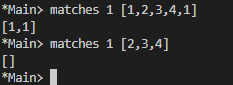
\includegraphics[width=8cm]{img/06.png}
\end{center}
Using matches or otherwise (\textbf{Hint: }e.g. the \textbf{patterns} functions seen in class), define a function 
\begin{lstlisting}
elem':: Integer -> [Integer] -> Bool  --elem is already defined in Prelude
\end{lstlisting}
which is True is the Integer is an element of the list, and False otherwise. 
\end{Exercise}
\begin{Answer}
\begin{lstlisting}
matches :: Eq a => a -> [a] -> [a]
matches x xs = [x' | x'<- xs, x == x']

--using matches
myElem :: Eq a => a -> [a] -> Bool
myElem x xs = matches x xs /=[]

--using patterns
myElem' :: Eq a => a -> [a] -> Bool
myElem' x xs = patterns x xs /=[]
\end{lstlisting}

\end{Answer}
\pagebreak
\begin{Exercise}
Suppose that a \textit{coordinate grid} of size $m$ \ $x$ \  $n$ is given by the list of all pairs $(x,y)$ of integers such that 
$ 0 \leq x \leq m $ and $ 0 \leq  y \leq n$. 
Using a list comprehension, define  a function:
\begin{center}
\begin{lstlisting}
grid :: Int -> Int -> [(Int, Int)]
\end{lstlisting}
\end{center}
that returns a coordinate grid of a given size. For example:
\begin{center}
	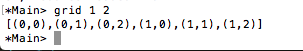
\includegraphics[width=8cm]{img/01.png}
\end{center}
\end{Exercise}
\begin{Answer}
  \begin{lstlisting}
    grid :: Int-> Int -> [(Int, Int)]
    grid x y = [(x', y')| x' <- [0..x], y'<- [0..y]]
    
  \end{lstlisting}
  
  \end{Answer}
\begin{Exercise}
Using a list comprehension and the function \textbf{grid} above, define a function 
\begin{lstlisting}
square :: Int ->  [(Int, Int)]
\end{lstlisting}
that returns a coordinate square of size n, excluding the diagonal from $(0,0)$ to $(n, n)$. For example: 
\begin{center}
	
\includegraphics[width=8cm]{img/02.png}
\end{center}
\end{Exercise}
\begin{Answer}
  \begin{lstlisting}
    square :: Int -> [(Int, Int)]
    square x = [(x', y')| x'<- [0..x], y' <- [0..x], x' /= y']
  \end{lstlisting}
  
  \end{Answer}

\begin{Exercise}
In a similar way to the function \textbf{\textit{length}}, show how the library function 
\begin{lstlisting}
replicate :: Int -> a -> [a]
\end{lstlisting}
that produces a list of identical elements can be defined using list comprehension. (Call your version \textbf{myReplicate}) 
For example: 
 \begin{center}
	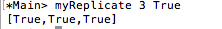
\includegraphics[width=8cm]{img/03.png}
\end{center} 
\end{Exercise}
\begin{Answer}
\begin{lstlisting}
myReplicate :: Int -> a -> [a]
myReplicate x y = [y| _ <- [1..x]]
\end{lstlisting}
\end{Answer}
\pagebreak
\begin{Exercise}
A triple $(x,y,z)$ of positive integers is called pythagorean if $x^2 + y^2 = z^2$.  Using a list comprehension, define a function
\begin{lstlisting}
pyths :: Int -> [(Int,Int,Int)]
\end{lstlisting}
that returns a list of all such triples whose components are at most a given limit. For example
\begin{center}
	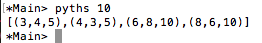
\includegraphics[width=8cm]{img/04.png}
\end{center}
\end{Exercise}
\begin{Answer}
\begin{lstlisting}
  pyths ::Int -> [(Int, Int, Int)]
  pyths n =  [(x, y,z) | x <- [1..n], y<- [1..n], z <- [1..n], x^2 + y^2 == z^2]
\end{lstlisting}
\end{Answer}
\begin{Exercise}
A positive integer is perfect if it equals the sum of all of its factors, excluding the number itself.  Using a list comprehension and the function \textbf{factors}, define a function
\begin{lstlisting}
perfects :: Int -> [Int]
\end{lstlisting}
that returns the list  of all perfect numbers up to a given limit. For example:
\begin{center}
	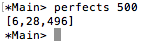
\includegraphics[width=8cm]{img/05.png}
\end{center}
\textbf{Hint: } Note that the list of factors of x includes x...
\end{Exercise}

\begin{Answer}
\begin{lstlisting}
  factors :: Int -> [Int]
  factors n = [x | x <- [1..n], n `mod` x ==0]
  
  perfects :: Int -> [Int]
  perfects n = [x | x <- [1..n], x == sum (factors x) - x]
  
  perfects' :: Int -> [Int]
  perfects' n = [x | x <- [1..n], x == sum ( init (factors x))]
\end{lstlisting}
\end{Answer}

\end{document}
